\chapter{Dr Kellogg i doktryna o Trójcy}

Kluczowym problemem kontrowersji  Kellogga były poglądy dotyczące \emcap{osobowości Boga}, które odchodziły od fundamentu naszej wiary, jakie Bóg ustanowił na początku naszej pracy. Powiedziano nam, że \egwinline{Wiele podobnych rzeczy pojawi się w przyszłości}[Ms137-1903.10; 1903][https://egwwritings.org/?ref=en\_Ms137-1903.10&para=9939.17]. W książce The Living Temple widzimy poglądy dotyczące \emcap{osobowości Boga} i miejsca Jego obecności, które odstępowały od \emcap{Fundamentalnych Zasad}. Ten krok nigdy nie powinien być wykonany! Nasuwa się jednak pytanie, dokąd ten krok zmierzał? Zobaczmy dowody na to, że ten krok zmierzał w kierunku doktryny o Trójcy. Siostra White prorokowała, że krok Kellogga doprowadzi do herezji Omega. Czy widzimy związek między sporem Kellogga a doktryną o Trójcy?

W poniższej sekcji chcemy przedstawić związek między sporem Kellogga a doktryną o Trójcy. Ważne jest podkreślenie, że The Living Temple nie zawiera tej doktryny w takiej formie, w jakiej jest ona dziś wyznawana. Głównym problemem w nauczaniu Kellogga było \textit{odstąpienie} od \emcap{Fundamentalnych Zasad}, które stanowiły fundament naszej wiary. Informacje, które przedstawimy, ujawniają, że dr Kellogg usprawiedliwiał swoje odstąpienie od fundamentalnych zasad wiary poprzez wiarę w doktrynę o Trójcy. Nie jest to trudne do zauważenia, gdy uznamy, że \emcap{Fundamentalne Zasady} były nie-trynitarne. Naszym głównym celem nie powinno być rozpoznawanie doktryny o Trójcy w argumentach Kellogga, ale raczej zrozumienie różnic między nauczaniem Kellogga a nauczaniem \emcap{o Fundamentalnych Zasadach naszej wiary} dotyczących \egwinline{osobowości Boga i miejsca Jego obecności}[SpTB02 51.3; 1903][https://egwwritings.org/?ref=en\_SpTB02.51.3&para=417.262]. Innymi słowy, jakie kroki podjął Kellogg odstępując od fundamentu naszej wiary? To podejście jest zalecane przez Ducha Proroctwa i pomoże nam uniknąć spekulacji dotyczących motywów Kellogga—pomoże nam skupić się na prawdzie. Ellen White mówi nam, że w The Living Temple jest wiele dobrych rzeczy, ale są one zmieszane ze zwodniczymi, podstępnymi teoriami dotyczącymi \emcap{osobowości Boga} i \emcap{Chrystusa}.

\begin{figure}[hp]
    \centering
    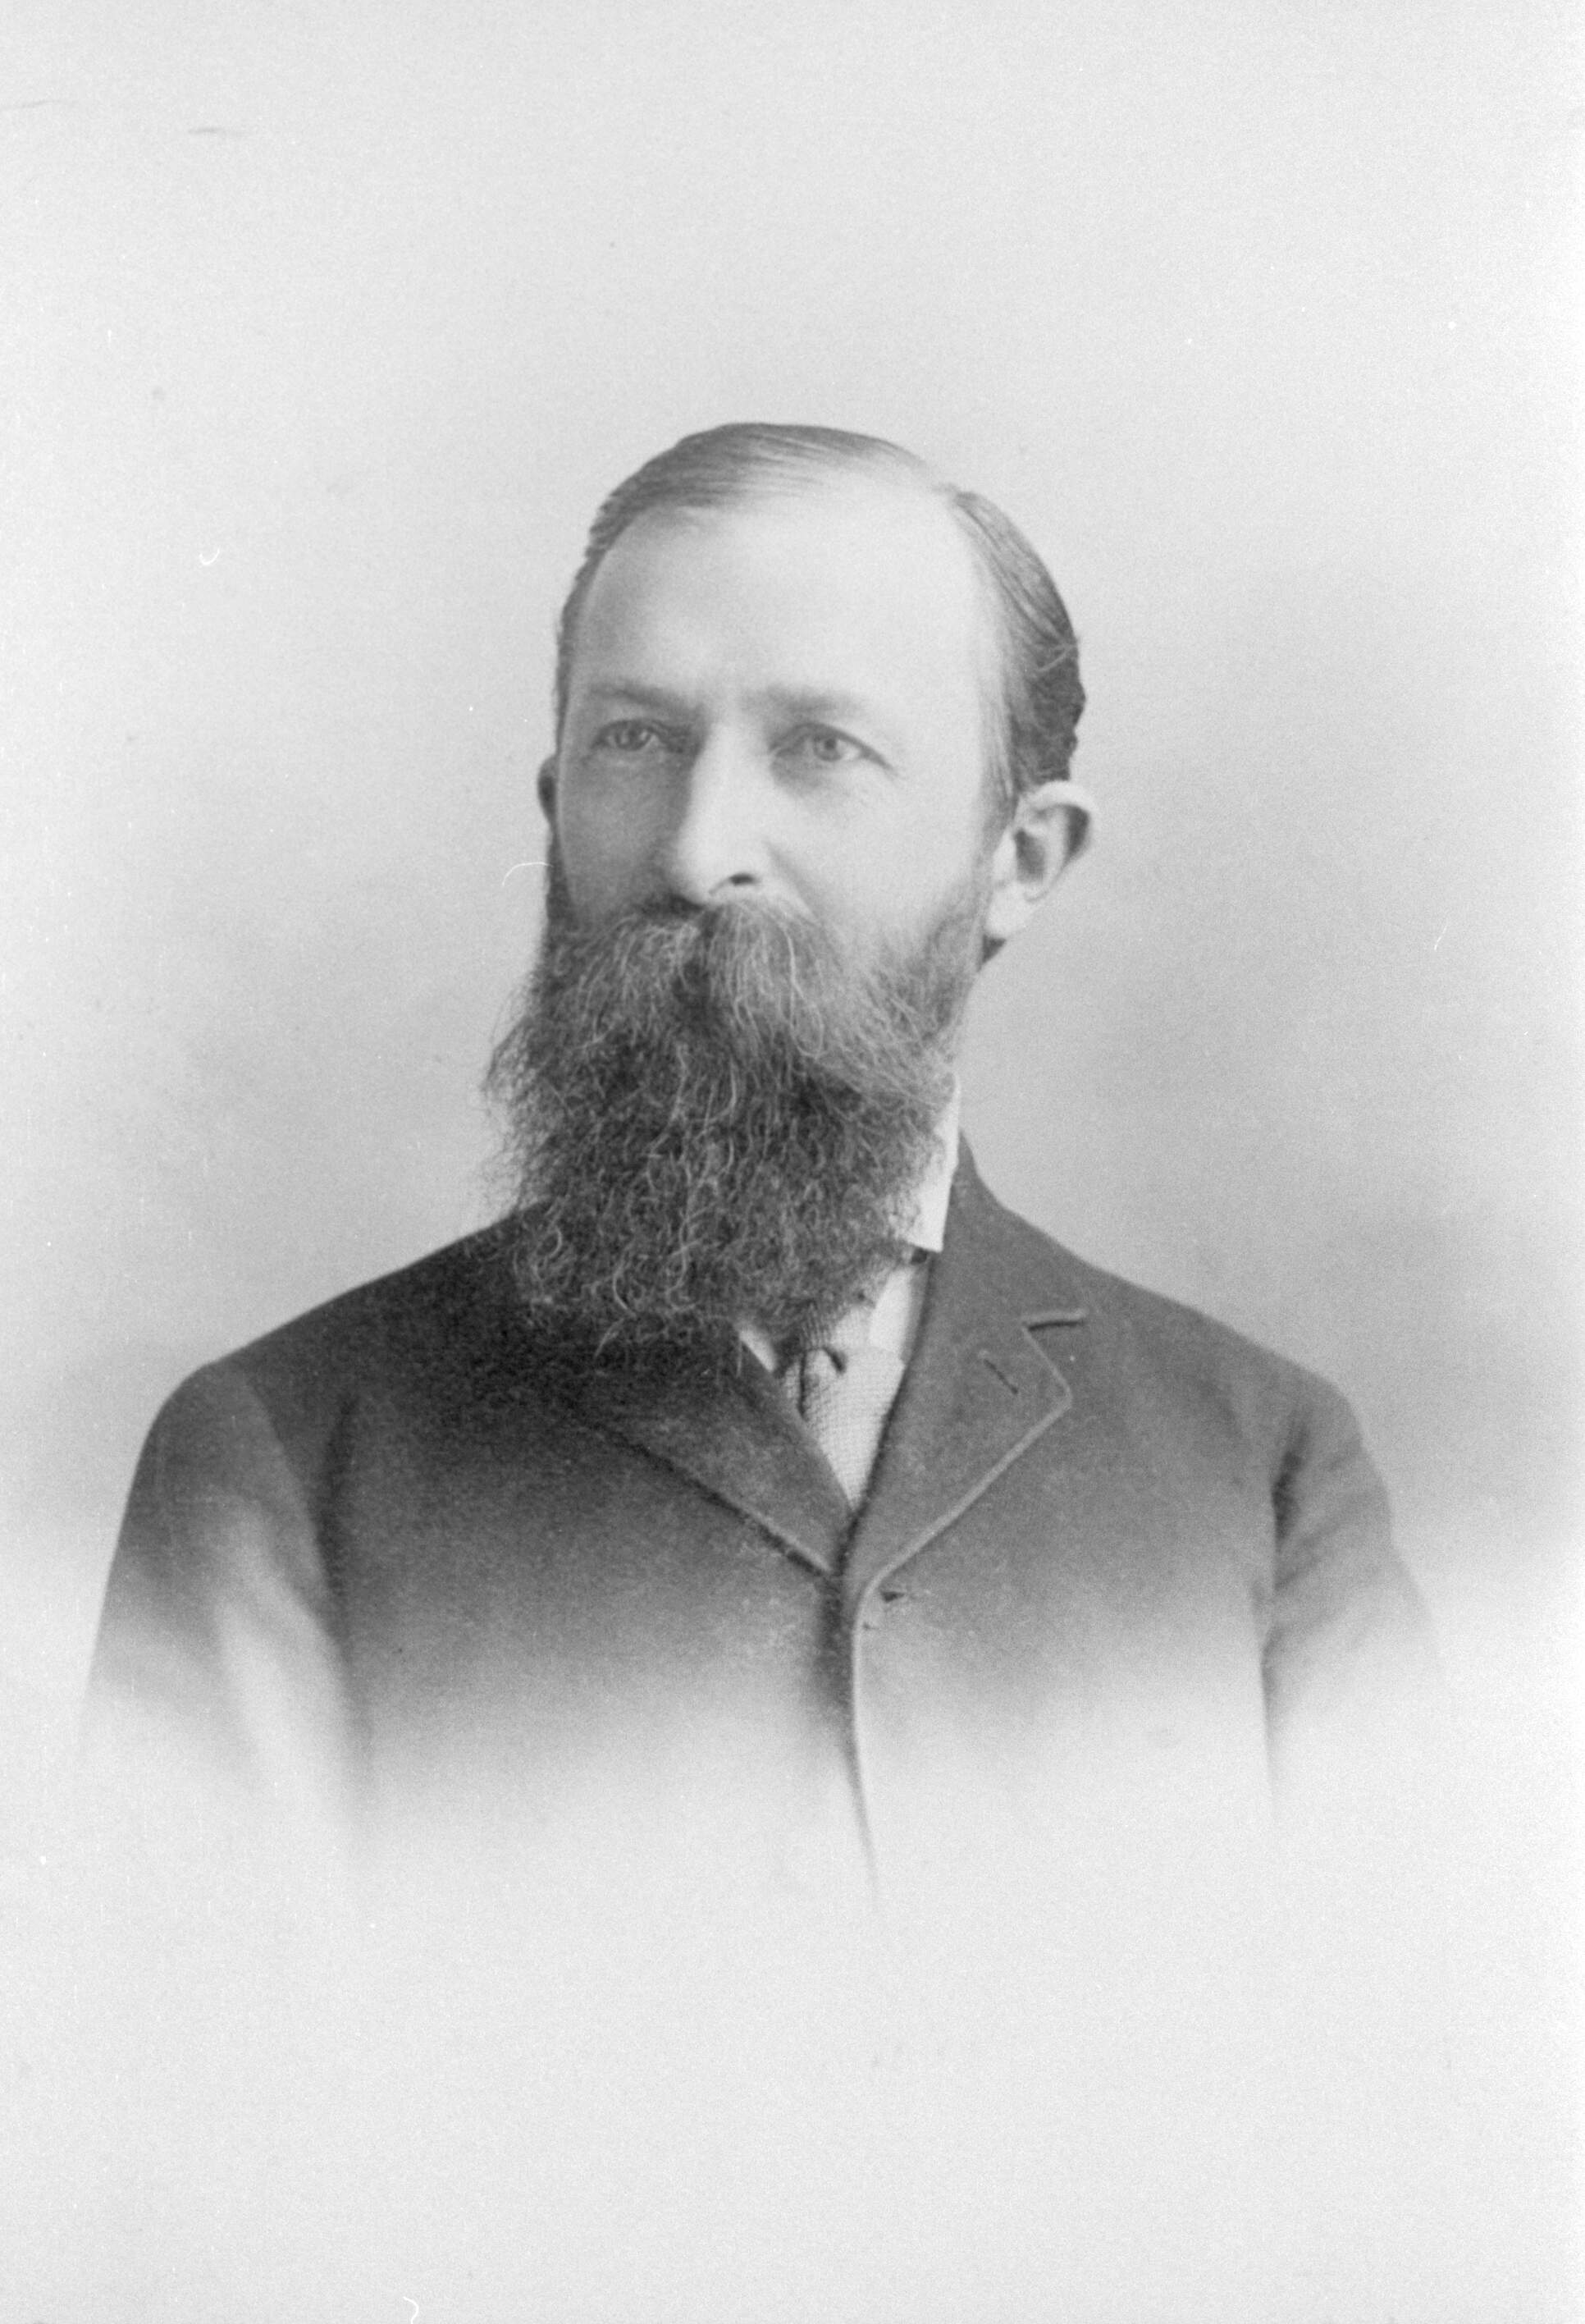
\includegraphics[width=1\linewidth]{images/john-h-kellogg.jpg}
    \caption*{John Harvey Kellogg (1852-1943)}
    \label{fig:john-h-kellogg}
\end{figure}

\egw{\textbf{Książka The Living Temple zawiera zwodnicze, \underline{podstępne poglądy dotyczące osobowości Boga i Chrystusa}}. Pan otworzył przede mną prawdziwe znaczenie tych poglądów, pokazując mi, że jeśli nie zostaną one stanowczo odrzucone, zwiodą nawet wybranych. \textbf{Cenna prawda i piękne poglądy zostały splecione z fałszywymi, wprowadzającymi w błąd teoriami. W ten sposób prawda została użyta do poparcia \underline{najbardziej niebezpiecznych błędów}. Cenne oświadczenia Boga są tak błędnie interpretowane, że wydają się popierać fałszerstwa \underline{zapoczątkowane przez wielkiego odstępcę}. Poglądy należące do objawień Boga są zmieszane ze zwodniczymi, podstępnymi teoriami szatańskich agencji}.}[Lt146-1905.2; 1905][https://egwwritings.org/?ref=en\_Lt146-1905.2&para=9430.8]

\egwnogap{W kontrowersji dotyczącej tej teorii\textbf{ twierdzono, że wierzyłam i nauczałam tych samych rzeczy}, które zostałam pouczona potępić w książce The Living Temple. \textbf{Zaprzeczam temu}. W imię Jezusa Chrystusa z Nazaretu, \textbf{mówię, że tak nie jest}.}[Lt146-1905.3; 1905][https://egwwritings.org/?ref=en\_Lt146-1905.3&para=9430.9]

To połączenie prawdy i błędu sprawia, że sprawa jest trudna. W oczach pro-trynitarnych uczonych problem jest przypisywany wyłącznie panteizmowi, a dowody na wiarę Kellogga w doktrynę o Trójcy są interpretowane jako wiara w fałszywą Trójcę\footnote{Whidden, Woodrow W, et al. \textit{The Trinity : Understanding God's Love, His Plan of Salvation, and Christian Relationships}. Hagerstown, Md, Review And Herald Pub. Association, 2002., p. 217}. Nagana Siostry White jest przypisywana obronie “prawidłowej” Trójcy, w którą rzekomo wierzyła. Niestety, taka interpretacja nie uznaje obrony przez Siostrę White \emcap{Fundamentalnych Zasad} dotyczących \emcap{osobowości Boga} i Chrystusa, więc jest błędną interpretacją jej prac. W następnych sekcjach zbadamy dane historyczne dotyczące związku dr Kellogga z doktryną o Trójcy z perspektywy adwentystycznej prawdy o \emcap{osobowości Boga}, co stanowiło fundament naszej wiary. Z tej perspektywy wierzymy, że dane historyczne zajaśnieją w nowym świetle i wywołają szczery i konstruktywny dialog w naszym kościele.

\section*{Korespondencja dr Kellogga i Brata Butlera}

W poniższej sekcji krótko przedstawiamy znaną korespondencję między dr Kelloggiem a G. I. Butlerem dotyczącą książki The Living Temple. Tutaj widzimy zastrzeżenia dr Kellogga dotyczące sporu. Napisał on do Brata Butlera:

\others{O ile mogę zgłębić, \textbf{trudność}, która znajduje się \textbf{w ‘The Living Temple’,} \textbf{całość można sprowadzić do pytania}: \textbf{\underline{Czy Duch Święty jest osobą}?} Ty mówisz nie. Przypuszczałem, że Biblia to stwierdza z tego powodu, ponieważ zaimek osobowy ‘on’ jest używany mówiąc o Duchu Świętym. \textbf{Siostra White używa zaimka ‘on’ i powiedziała dosłownie, że Duch Święty jest \underline{trzecią osobą Bóstwa}}. \textbf{Jak Duch Święty może być trzecią osobą i wcale nie być osobą, trudno mi zrozumieć}.}[Letter: J. H. Kellogg to G. I. Butler. Oct 28. 1903][https://static1.squarespace.com/static/554c4998e4b04e89ea0c4073/t/5db9fbc96defed1e45b497a4/1572469707862/1903-10-28-Kellog-to-Butler.pdf]

\begin{figure}[hp]
    \centering
    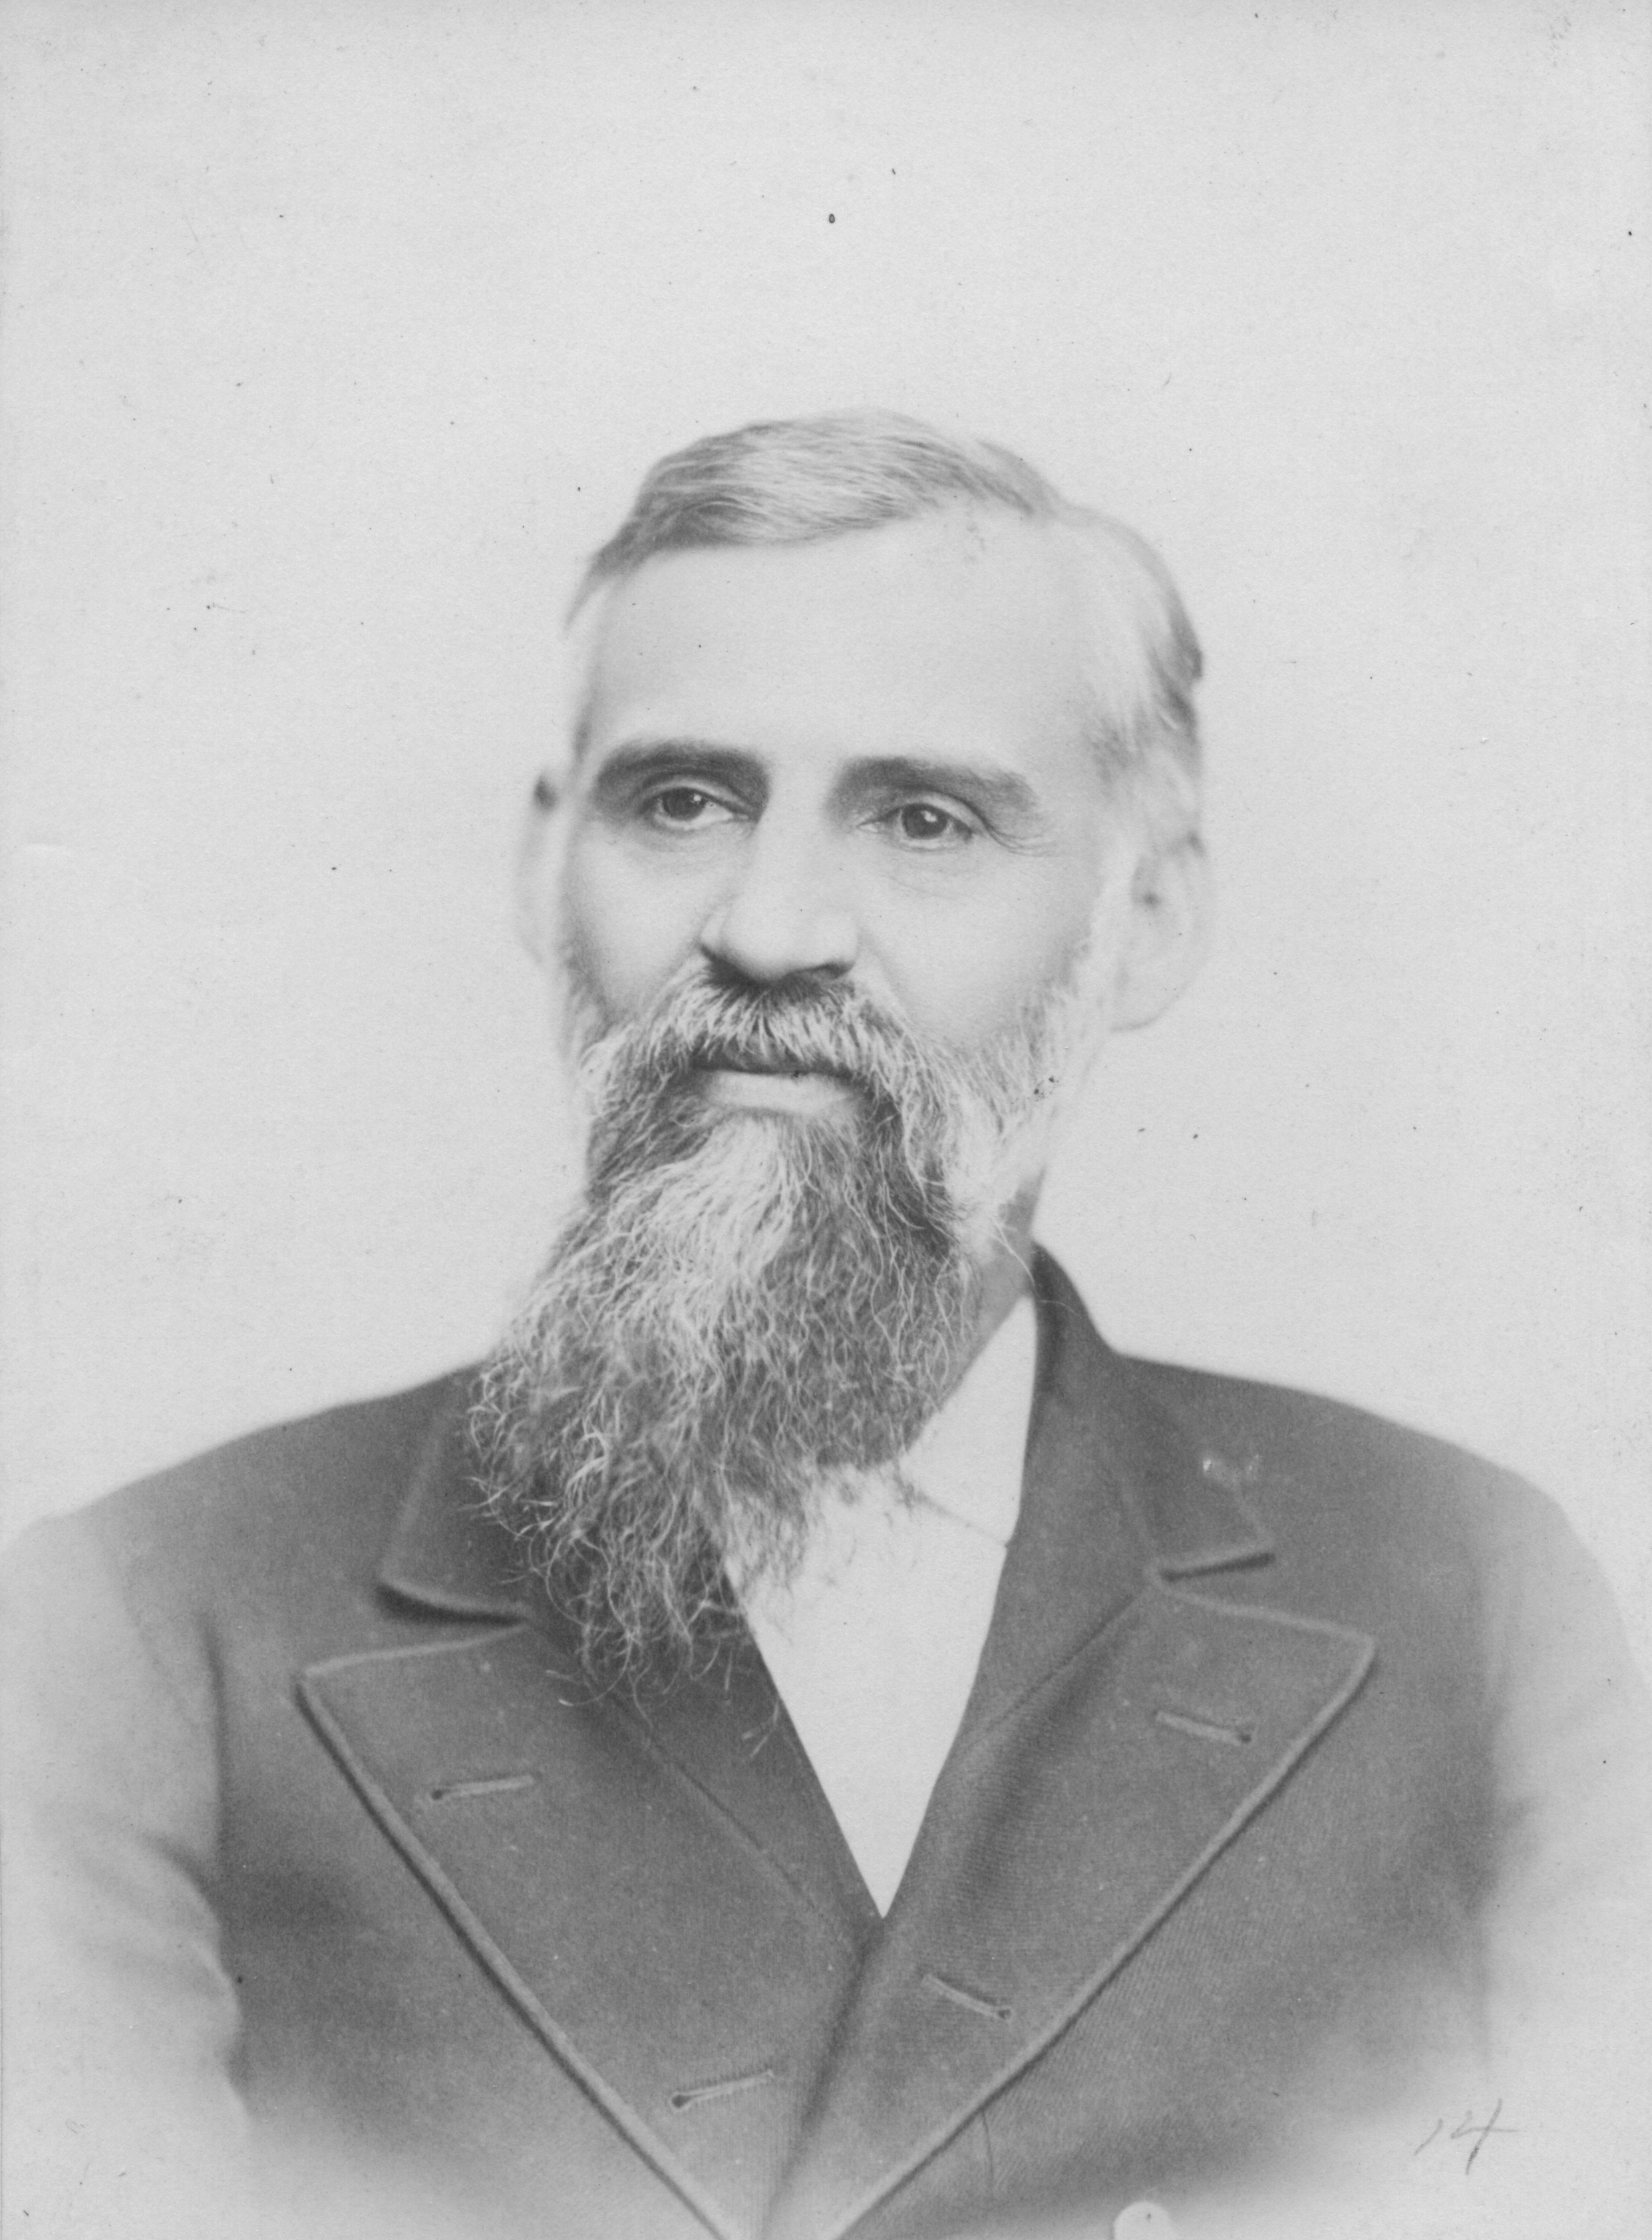
\includegraphics[width=1\linewidth]{images/george-ide-butler.jpg}
    \caption*{George Ide Butler (1834-1918)}
    \label{fig:g-i-butler}
\end{figure}

Według perspektywy dr Kellogga, cały problem z książką ‘The Living Temple’ sprowadza się do pytania “\textit{Czy Duch Święty jest osobą?}”. Oczywiście nie opowiada się on za bezosobowym Bogiem, jak jest często oskarżany\footnote{Whidden, Woodrow W, et al. \textit{The Trinity : Understanding God's Love, His Plan of Salvation, and Christian Relationships}. Hagerstown, Md, Review And Herald Pub. Association, 2002.,str.217}. Co więcej, wierzy nawet, że Duch Święty jest \textit{trzecią osobą Bóstwa}. Twierdzi też, że Brat Butler nie wierzy, że Duch Święty jest osobą. Problem najwyraźniej leży w definicji słowa \textit{‘osoba’}. W tym punkcie Kellogg kontynuuje:

\others{Wierzę, że ten Duch Boży jest osobowością, ty nie. Ale to jest czysto kwestia definicji. \textbf{Wierzę, że Duch Boży jest osobowością}; ty mówisz: Nie, to nie jest osobowość. Teraz jedynym powodem, dla którego się różnimy, jest to, że \textbf{różnimy się w naszych poglądach co do tego, \underline{czym jest osobowość}}. \textbf{Twoje pojęcie osobowości to być może \underline{podobieństwo do osoby} lub istoty ludzkiej}.}[Letter: J. H. Kellogg to G. I. Butler. Oct 28. 1903][https://static1.squarespace.com/static/554c4998e4b04e89ea0c4073/t/5db9fbc96defed1e45b497a4/1572469707862/1903-10-28-Kellog-to-Butler.pdf]

Brat Butler odpowiedział:

\others{\textbf{Jak dotąd  Siostra White i ty jesteście w pełnej zgodzie, będę musiał pozostawić to całkowicie między tobą a Siostrą White. \underline{Siostra White mówi, że nie ma pełnej zgodności; ty twierdzisz, że jest}. \underline{Wiem, że niektóre jej uwagi wydają się dawać ci mocne podstawy do twierdzenia, że tak jest}. Jestem na tyle szczery, by to przyznać, ale muszę dać jej wiarę, dopóki sama temu nie zaprzeczy, że mówi też o różnicy, i nie sądzę, żebyś mógł w pełni zrozumieć, co ma na myśli. \underline{Bóg mieszka w nas przez swojego Ducha Świętego}, jako Pocieszyciel, jako Ten, który napomina, a w szczególności to pierwsze. Kiedy przychodzimy do Niego, uczestniczymy w Nim w tym sensie, że Duch pochodzi od Niego; \underline{pochodzi od Ojca i Syna}. Nie jest to osoba chodząca pieszo lub latająca \underline{jako dosłowna istota}, \underline{w takim sensie jak Chrystus i Ojciec} – a przynajmniej, jeśli tak jest, to całkowicie wykracza to poza moje rozumienie znaczenia języka czy słów}.}[Letter: G. I. Butler to J. H. Kellogg. April 5. 1904]

Ta otrzymana korespondencja jest kluczowa w zrozumieniu sporu Kellogga. Sam Kellogg stwierdził, \others{całą sprawę można sprowadzić do pytania: \textbf{Czy Duch Święty jest osobą?}} Podobnie dr Kellogg napisał do Williama White'a: \others{Bardzo uważnie studiowałem, aby zobaczyć, jaki jest \textbf{prawdziwy rdzeń problemu z The Living Temple}, i o ile mogę dostrzec, \textbf{\underline{całe zagadnienie} sprowadza się do tego: \underline{Czy Duch Święty jest osobą}?}}[Letter J. H. Kellogg to William White, October 28, 1903][https://drive.google.com/file/d/1\_S4S-Hc0K7Ka8gda9oRhPuAb9XzBTwmb/view] Jak wniosek Kellogga ma się do przeglądu i instrukcji niebiańskiego pochodzenia, który wyraźnie nam mówi,że rozumowanie w The Living Temple jest \egwinline{niczym innym jak spekulacją odnośnie \textbf{osobowości Boga i tego gdzie jest jego obecność}}[SpTB02 51.3; 1904][https://egwwritings.org/?ref=en\_SpTB02.51.3&para=417.262]? W pismach Ellen White i pionierów termin ‘\textit{osobowość Boga}’ odnosi się konkretnie do osobowości Ojca. Dlaczego więc Kellogg twierdzi, że prawdziwym problemem jest osobowość Ducha Świętego, podczas gdy Bóg wskazał, że problem dotyczy osobowości Ojca?

Wielu zakłada, że dr Kellogg manipuluje, uchylając się od sedna sprawy. Jednak przy pewnym założeniu jego argumenty dotyczące osobowości Ducha Świętego logicznie wspierają jego kontrowersyjne poglądy na temat \emcap{osobowości Boga}. To założenie staje się widoczne w samych danych, gdy uważnie śledzimy jego sposób rozumowania.

Jak widzieliśmy wcześniej, doktryna o \emcap{osobowości Boga} naucza, że Bóg Ojciec posiada formę—namacalne, materialne ciało. Dr Kellogg zgodził się, że to twierdzenie jest prawdziwe w granicach naszej ograniczonej koncepcji pojmowania Boga\footnote{\href{https://archive.org/details/J.H.Kellogg.TheLivingTemple1903/page/n33/}{Dr. John H. Kellogg, The Living Temple, str.31.}}. Jednak argumentował, że w rzeczywistości Bóg wykracza poza nasze koncepcje dotyczące Jego formy, ponieważ jest poza ograniczeniami przestrzeni\footnote{\href{https://archive.org/details/J.H.Kellogg.TheLivingTemple1903/page/n33/}{Dr. John H. Kellogg, The Living Temple, str.33.}}. W tym sensie Kellogg skutecznie eliminuje rzeczywistość fizycznego, materialnego ciała Boga. Założeniem, które uzasadniałoby punkt widzenia dr. Kellogga, jest \textit{wyłączna równoważność} w rozumieniu \emcap{osobowości Boga} i osobowości Ducha Świętego. Czy Duch Święty jest ograniczony przestrzenią? Nie, nie jest. Czy Duch Święty ma fizyczne ciało? Nie! Według Jezusa, \bible{duch nie ma ciała ani kości}[Łk 24:39]. Czy Duch Święty jest osobą? Odpowiedź zależy od naszej interpretacji tego, co to znaczy być osobą. Jaka jest właściwość lub stan Ducha Świętego jako osoby?\footnote{Bezpośrednie zastosowanie definicji słowa ‘\textit{osobowość}’ ze \href{https://www.merriam-webster.com/dictionary/personality}{Słownika Merriam Webster}} Porównując wiarę dr. Kellogga w osobowość Ducha Świętego z poglądami Brata Butlera, staje się oczywiste, że właściwość Ducha Świętego jako osoby nie jest zgodna z \others{tym \textbf{podobieństwem do osoby} lub istoty ludzkiej}. Butler wyraźnie określił swoje kryteria dla tego postanowienia\footnote{W swoim liście do dr. Kellogga, Brat Butler dalej stwierdził, że nie ma rozróżnienia między osobą a cielesną obecnością. Zobacz \href{https://c7da.us/egwdl/Butler\%20to\%20Kellogg\%20Aug121904.pdf}{List od Butlera do Kellogga, 12 sierpnia 1904, str.6}}: \others{\textbf{To nie jest osoba chodząca pieszo lub latająca \underline{jako dosłowna istota}, \underline{w takim sensie jak Chrystus i Ojciec} – a przynajmniej, jeśli tak jest, to całkowicie wykracza to poza moje pojmowanie języka czy słów}}.

Czy zauważyłeś, że Brat Butler odniósł się do niewypowiedzianego założenia Kellogga? Butler nakreślił rozróżnienie między Ojcem i Chrystusem w stosunku do Ducha Świętego. Brat Butler ma rację. Istnieje kontrast między osobowością Ducha Świętego a osobowością Boga i Chrystusa. Chrystus i Ojciec posiadają fizyczną formę osoby, podczas gdy Duch Święty nie. Odrzucenie fizycznej formy osoby Ojca oznacza \textit{całkowite zrównanie} rozumienia osobowości Ojca z osobowością Ducha Świętego. Podejście Kellogga jest przekonujące, ponieważ było poparte ważnymi argumentami dotyczącymi osobowości Ducha Świętego.

Przyjrzyjmy się krótko osobowości Ducha Świętego. Jaka jest właściwość lub stan Ducha Świętego jako osoby?

\egw{\textbf{Duch Święty ma osobowość}, \textbf{\underline{inaczej}} nie mógłby \textbf{świadczyć} naszemu duchowi i z naszym duchem, że jesteśmy dziećmi Bożymi. \textbf{Musi On być również \underline{boską osobą}}, \textbf{\underline{inaczej}} nie mógłby \textbf{badać tajemnic}, które są ukryte \textbf{w umyśle Boga}.}[21LtMs, Ms 20, 1906, par. 32; 1906][https://egwwritings.org/read?panels=p14071.10296041&index=0]

\egw{\textbf{Duch Święty jest osobą}; \textbf{\underline{ponieważ}} On \textbf{świadczy} z naszym duchem, że jesteśmy dziećmi Bożymi.}[21LtMs, Ms 20, 1906, par. 31; 1906][https://egwwritings.org/read?panels=p14071.10296040&index=0]

Cechy lub stany, które określają Ducha Świętego jako osobę, są wyraźnie wymienione w przytoczonych cytatach. Obejmują one zdolność do składania świadectwa i badania umysłu. Dalsze potwierdzenie można znaleźć w Piśmie Świętym, które przypisuje Duchowi Świętemu działania takie jak mówienie (\textit{Dzieje 13:2}), nauczanie (\textit{Jan 14:26; 1 Koryntian 2:13}), podejmowanie decyzji (\textit{Dzieje 15:28}) i doświadczanie emocji (\textit{Efezjan 4:30}), pośród innych. Te \textit{cechy} wspólnie potwierdzają osobowość Ducha Świętego. Czy te same cechy można również przypisać Ojcu i Synowi? Z całą pewnością. Jednak w przeciwieństwie do Ojca i Syna, Duch Święty wyróżnia się brakiem materialnej, namacalnej formy. Kiedy Ellen White pytała Chrystusa o \emcap{osobowość Boga}, jej pytanie konkretnie dotyczyło osobowej formy jako definiującej cechy osobowości Ojca.

\egw{Często \textbf{widziałam} kochanego  Jezusa, że \textbf{jest On osobą}. \textbf{Zapytałam Go, czy Jego Ojciec \underline{jest osobą} i \underline{ma postać} jak On}. Jezus odpowiedział: «\textbf{Jestem dokładnym odbiciem osoby Mojego Ojca}»}[EW 77.1; 1882][https://egwwritings.org/read?panels=p28.490&index=0]

To prowadzi nas do głębokiej różnicy w sposobie rozumienia osobowości Ducha Świętego w przeciwieństwie do Ojca i Syna. Ellen White opisuje Ducha Świętego jako duchową manifestację Chrystusa, wyraźnie rozróżniając między zewnętrzną, widzialną manifestacją Chrystusa a Jego duchową manifestacją. Ten kontrast podkreśla wyjątkową naturę obecności i działania Ducha Świętego na świecie, odmienną od fizycznej obecności Chrystusa i Ojca. Zwróć uwagę na kontrast między zewnętrzną, widzialną manifestacją Chrystusa a Jego duchową manifestacją:

\egw{\textbf{Chrystus} miał \textbf{objawić się} im, a jednak \textbf{być niewidzialnym dla świata}, było to tajemnicą dla uczniów. Nie mogli zrozumieć \textbf{słów Chrystusa w ich \underline{duchowym sensie}}. \textbf{Myśleli o \underline{zewnętrznej, widzialnej manifestacji}}. Nie mogli pojąć faktu, że mogą być \textbf{w obecności Chrystusa }, a \textbf{jednocześnie może być On niewidzialny dla świata}. \textbf{Nie rozumieli znaczenia \underline{duchowej manifestacji}}.}[ST November 18, 1897, par. 6; 1897][https://egwwritings.org/read?panels=p820.14727&index=0]

Duch Święty nie jest osobą w sensie fizycznym, ale objawia się w sensie duchowym. Jeśli wyłączne rozumienie osobowości Ducha Świętego zostanie zastosowane do Ojca, to w konsekwencji Jego fizyczna forma osoby zostaje zniesiona. Jego osobowość jest uduchowiona. Dlatego Ellen White krytycznie określiła perspektywę Kellogga jako spirytualizm. Czy wiesz, która doktryna w szczególności ma podstawową zasadę, że Ojciec i Duch Święty są równi w swoich osobowościach? Jest to \textit{doktryna o Trójcy}. Czy możliwe, że Dr. Kellogg faktycznie poruszał teologiczną stroną pytań o Trójcę?

\section*{Wyznanie Kellogga o The Living Temple}

W swoim wywiadzie z G. W. Amadonem i A. C. Bourdeau, miesiąc po wykluczeniu z kościoła, wyznał, że nieumyślnie wprowadził teologiczną stronę kwestii Trójcy do swojej książki “The Living Temple”.

\others{\textbf{Teraz, myślałem, że całkowicie usunąłem stronę teologiczną kwestii \underline{Trójcy i wszystkich tego typu rzeczy}}. \textbf{Nie zamierzałem \underline{tego umieszczać}} w ogóle, i zadbałem o to, aby stwierdzić to w przedmowie. Nigdy nie śniło mi się o \textbf{jakiejkolwiek kwestii teologicznej} \textbf{\underline{wprowadzonej do tego}}. Chciałem tylko pokazać, że \textbf{serce nie bije samo z siebie, ale że to moc Boża utrzymuje je w ruchu}.}[Kellogg vs. The Brethren: His Last Interview as an Adventist, str. 58.][https://forgotten-pillar.s3.us-east-2.amazonaws.com/1990\_kellogg\_vs\_brethren\_lastInterview\_oct7\_1907\_spectrum\_v20\_n3-4.pdf]

Gdybyśmy mieli szukać w jego książce trynitarnych wyrażeń, nie znaleźlibyśmy ich. Czy byłby to dowód, że Kellogg jest nieszczery w swoim wyznaniu? Jedyne, co znajdujemy, to nauczanie, które odchodzi od fundamentu naszej wiary—\emcap{fundamentalnych zasad}—dotyczących \emcap{osobowości Boga} i gdzie jest Jego obecność. Trynitarne wyrażenia nie są tam obecne, ale jego poglądy dotyczące \emcap{osobowości Boga} są zgodne z trynitarnymi poglądami na temat osobowości Boga. Te poglądy są zwodnicze i Kellogg został za nie zganiony. Kiedy chciał wyraźnie stwierdzić wiarę w doktrynę o Trójcy, mając nadzieję na poprawienie książki, został ponownie zganiony słowami, \egwinline{\textbf{Łatane teorie} nie mogą być przyjęte przez tych, którzy są lojalni wobec wiary} i wobec \emcap{Fundamentalnych Zasad}\footnote{\href{https://egwwritings.org/?ref=en_Lt253-1903.28&para=9980.36}{EGW, Lt253-1903.28; 1903}}. Kluczowym problemem doktryny o Trójcy, w odniesieniu do \emcap{osobowości Boga}, jest podstawowe założenie, że wszyscy Trzej, Ojciec, Syn i Duch Święty, posiadają ten sam rodzaj osobowości w taki sposób, że tworzą jednego monoteistycznego Boga. W tym świetle możemy zrozumieć twierdzenia Kellogga dotyczące osobowości Ducha Świętego, że Duch Święty jest trzecią osobą Bóstwa. Dr Kellogg cytował Ellen White, gdy wysuwał swoje twierdzenia; chociaż używał tych samych słów, miał błędny pogląd. W świetle wyznania Dr. Kellogga o włączeniu \others{\textbf{teologicznej strony pytań o \underline{Trójcę}}}, i jego twierdzenia, że \others{\textbf{całą tę sprawę można sprowadzić do pytania}: \textbf{\underline{Czy Duch Święty jest osobą}}?}, możemy dostrzec niewypowiedziane założenie, że Ojciec i Syn są w taki sam sposób osobami jak Duch Święty. Dlatego Brat Butler napisał do niego odnośnie osobowości Ducha Świętego: \others{\textbf{To nie jest osoba chodząca dookoła pieszo, ani latająca \underline{jako dosłowna istota}, \underline{w takim sensie jak Chrystus i Ojciec są} – przynajmniej, jeśli tak jest, to całkowicie przekracza to moje rozumienie pojmowania języka czy słów.}}[List od G. I. Butlera do J. H. Kellogga, 5 kwietnia 1904.]

\section*{Obecność Boga objawiona w naturze}

Z dzieł naszych pionierów widzieliśmy, że osobowość Ducha Świętego jest najwyraźniej wyrażona w kategoriach obecności Boga. Siostra White powiedziała nam, że The Living Temple \egwinline{wprowadza to, co jest jedynie spekulacją odnośnie \textbf{osobowości Boga i miejsca Jego obecności}.}[SpTB02 51.3; 1904][https://egwwritings.org/?ref=en\_SpTB02.51.3&para=417.262] \emcap{Osobowość Boga} i miejsce Jego obecności to dwie wzajemnie powiązane doktryny; jedna potwierdza drugą. Zaprzeczając jednej, zaprzeczysz i drugiej. Ta koncepcja jest wyraźnie widoczna w książce The Living Temple. W poprzednich sekcjach czytaliśmy argumenty Kellogga dotyczące \emcap{osobowości Boga} zaczerpnięte z jego książki. Twierdził, że bezużyteczne jest mówienie o kształcie Boga czy jakiejkolwiek namacalnej formie. Wzbudził sceptycyzm co do rzeczywistości Boga jako określonej, materialnej i namacalnej Istoty. Jeśli Bóg jest duchem, nie posiadającym formy ani ciała, to nie jest ograniczony w swojej obecności do jednego miejsca; taki był pogląd, który Kellogg propagował w The Living Temple.

\others{Ktoś mówi: ‘\textbf{Bóg może być \underline{obecny przez swojego Ducha} lub przez swoją moc, ale \underline{z pewnością sam Bóg} nie może być obecny wszędzie naraz}.’ Odpowiadamy: Jak można oddzielić moc od źródła mocy? \textbf{Gdzie Duch Boży działa}, gdzie objawia się Boża moc, \textbf{tam \underline{sam} Bóg jest rzeczywiście i prawdziwie obecny}...}[John H. Kellogg, The Living Temple, str.28.][https://archive.org/details/J.H.Kellogg.TheLivingTemple1903/page/n29/]

Kiedy dr Kellogg napisał \others{Ktoś mówi: ‘Bóg może być obecny przez swojego Ducha...’}, odnosił się do poglądów naszych pionierów, którzy byli wierni \emcap{Fundamentalnym Zasadom}. Jest to najbardziej oczywisty punkt, w którym dr Kellogg odstąpił od \emcap{Fundamentalnych Zasad}. Czy ten krok jest zgodny z doktryną o Trójcy? Badając nasze obecne stanowisko w Fundamentalnych Wierzeniach \#2, widzimy, że jeden Bóg, jako jedność trzech osób, nie jest wszędzie obecny poprzez działanie Ducha Świętego, ale raczej jest wszędzie obecny sam w sobie.

\others{Jest \textbf{jeden Bóg}: Ojciec, Syn i Duch Święty, \textbf{jedność trzech} współwiecznych \textbf{Osób}. Bóg jest nieśmiertelny, wszechmocny... i \textbf{zawsze obecny}.}[Fundamental Beliefs of Seventh-day Adventist, \#2 Trinity; 2020 Edition][https://www.adventist.org/wp-content/uploads/2020/06/ADV-28Beliefs2020.pdf]

\section*{Postrzeganie Boga przez dr. Kellogga}

Badając otaczający spór wokół The Living Temple, rzeczywiście widzimy, że dr Kellogg poruszył \others{teologiczną stronę kwestii trójcy.}[Kellogg vs. The Brethren: His Last Interview as an Adventist, p. 58.][https://forgotten-pillar.s3.us-east-2.amazonaws.com/1990\_kellogg\_vs\_brethren\_lastInterview\_oct7\_1907\_spectrum\_v20\_n3-4.pdf] Kolejne pytanie, które nam się nasuwa badając poglądy Kellogga w kontekście \emcap{Fundamentalnych Zasad}, to kogo ma na myśli mówiąc o “\textit{jednym Bogu}”? Nie ma bezpośrednich danych, by odpowiedzieć na to pytanie, ale jest wiele danych sugerujących, że rozumienie “\textit{jednego Boga}” przez dr. Kellogga było trynitarne. Jego list do W. W. Prescotta jest jednym z dowodów potwierdzających tę koncepcję:

\others{Różnica jest taka: \textbf{Kiedy mówimy Bóg} jest w drzewie, słowo ‘\textbf{Bóg}’ \textbf{jest rozumiane w jego najbardziej wszechstronnym znaczeniu}, i ludzie rozumieją, że oznacza to, że \textbf{Bóstwo} jest w drzewie, \textbf{Bóg Ojciec, Bóg Syn i Bóg Duch Święty}, podczas gdy właściwe zrozumienie, aby \textbf{ zachować zdrowy rozsądek } w naszych umysłach, jest takie, że Bóg Ojciec zasiada na swoim tronie w niebie, gdzie jest również Bóg Syn; \textbf{podczas gdy życie Boga, czyli duch lub obecność jest wszechprzenikającą mocą, która wypełnia wolę Boga w całym wszechświecie}.}[Letter: Dr. Kellogg to Prof. W. W. Prescott, Oct. 25, 1903][https://forgotten-pillar.s3.us-east-2.amazonaws.com/1903-10-25-JHKellogg-to-W.W.Prescott.pdf]

W następnym rozdziale przedstawimy naszą argumentację: jeśli dany \others{zdrowy rozsądek} odnośnie Boga propagowany przez dr. Kellogga był prawdziwy, to jego wyjaśnienie, że Duch Święty jest \others{życiem Boga, duchem lub obecnością, która jest wszechprzenikającą mocą wypełniającą wolę Boga w całym wszechświecie} rzeczywiście rozwiązałoby cały problem The Living Temple. Ale tak nie było. Prawdziwym problemem dr. Kellogga było jego postrzeganie Boga, a jego trynitarne stanowisko nie rozwiązywało rzeczywistego problemu—\emcap{osobowości Boga}.

Jest jeszcze jeden wymowny list pokazujący nam konsekwencje poruszając \others{teologiczną stronę kwestii dotyczących trójcy.} Pisząc do swojego przyjaciela dr. Haywarda, dr Kellogg zastanawiał się:

\others{\textbf{Ci teologowie} starali się zaciemnić umysły ludzi i sprawić, by \textbf{ta słodka i piękna prawda \underline{wydawała się} im \underline{odrażająca}, wciągając w nią \underline{stary spór o Trójcę}}.}

\othersnogap{Nigdy nie poruszałem kwestii \textbf{która część Boga jest obecna w człowieku}, czy to był \textbf{Bóg Ojciec}; \textbf{Bóg Syn}; czy \textbf{Bóg Duch Święty}. Jedynym punktem było to, że jest to Bóg, a nie człowiek.}[Letter: Dr. J. H. Kellogg to Dr. Hayward, Aug., 15. 1905][https://forgotten-pillar.s3.us-east-2.amazonaws.com/1903-08-15-kellogg-to-hayward.pdf]

Tutaj widzimy spięcia między dr. Kellogiem a pewnymi teologami Kościoła Adwentystów Dnia Siódmego z tamtego okresu, gdzie \others{słodka i piękna prawda} dr. Kellogga o boskiej immanencji zaplątała się w \others{stary spór o Trójcę}. Mówi nam to, że w czasach dr. Kellogga doktryna o Trójcy była kontrowersyjna i z pewnością nie była postrzegana jako coś pozytywnego, ale raczej jako coś, co czyniło nauki Kellogga \others{odrażającymi}. Ale kim byli ci teologowie, o których wspominał dr Kellogg? Nie wymienił nikogo w swoim liście do dr. Haywarda, ale możemy się domyślić, kim byli \others{ci teologowie} na podstawie jego listu wysłanego 10 dni wcześniej do I. G. Butlera\footnote{\href{https://forgotten-pillar.s3.us-east-2.amazonaws.com/1905-08-05-kellogg-butler.pdf}{Letter: J. H. Kellogg to I. G. Butler, Aug., 5. 1905}}, w którym wyraźił swoją frustrację wobec przetargów Generalnej Konferencji z nim. Byli to A. G. Daniells, W. C. White i W. W. Prescott. Możemy również włączyć do tej grupy samego G. I. Butlera, ponieważ on również był teologiem uczestniczącym w tym \others{starym sporze o Trójcę}. Wszyscy ci ludzie zajmowali czołowe stanowiska w Kościele Adwentystów Dnia Siódmego i wszyscy byli nie-trynitarianami. Pojawia się argument, że problem z nauczaniem dr. Kellogga leży gdzie indziej niż w jego trynitarnych poglądach, ponieważ rzekomo kościół był wtedy trynitarny, a Ellen White sama była trynitarianką.\footnote{Jest to obecnie główna narracja promowana przez naszych adwentystycznych uczonych.} Jeśli tak było, i w tej mieszaninie prawdy i błędu, czy nie powinniśmy mieć przynajmniej jakiejś obrony doktryny o Trójcy, oddzielającej ją od błędu? Nie znaleźliśmy takich danych. Zamiast tego, wszystkie dane, które mamy, są w obronie \emcap{Fundamentalnych Zasad} i doktryny o obecności i \emcap{osobowości Boga}, które obie są przeciwne doktrynie o Trójcy. Ellen White powiedziała o prawdzie: doktryna o Trójcy \egwinline{nie może być przyjęta przez \textbf{lojalnych wobec wiary i zasad}, które wytrzymały wszelki sprzeciw szatańskich wpływów.}[Lt253-1903.28; 1903][https://egwwritings.org/?ref=en\_Lt253-1903.28]

W tej krótkiej refleksji na temat różnic między poglądami dr. Kellogga a \emcap{Fundamentalnymi Zasadami}, od których odstąpił, możemy rozpoznać następujące cechy, które są pokrewne doktrynie o Trójcy:

\begin{itemize}
    \item Słowo ‘Bóg’ reprezentuje całościową koncepcję Boga jako Boga Ojca, Boga Syna i Boga Ducha Świętego.
    \item Bóg jest wszędzie obecny przez Siebie samego.
    \item Właściwość lub stan Ojca jako osoby jest zrównany z tym Ducha Świętego.\footnote{\href{https://www.adventist.org/wp-content/uploads/2020/06/ADV-28Beliefs2020.pdf}{Fundamental Beliefs \#5}: \others{On \normaltext{[Duch Święty]} \textbf{jest tak samo osobą} \underline{jak} \textbf{Ojciec} i Syn}; \href{https://www.adventist.org/wp-content/uploads/2020/06/ADV-28Beliefs2020.pdf}{Fundamental Beliefs \#3}: \others{\textbf{Cechy} i moce \textbf{przejawiające się w} Synu i \textbf{Duchu Świętym są \underline{również} cechami Ojca}}}
\end{itemize}

Te trzy cechy poglądów dr. Kellogga odbiegają od fundamentu naszej wiary—\emcap{Fundamentalnych Zasad}—ale są w harmonii z naukami o Trójcy. Mówiąc to, nie twierdzimy, że dr Kellogg jest odpowiedzialny za przyjęcie doktryny o Trójcy w nasze szeregi, ale raczej że doktryna o Trójcy była uzasadnieniem Kellogga dla odstąpienia od fundamentu naszej wiary, ustanowionego na początku naszej pracy. Prawdziwym problemem było \textit{odstąpienie} od \emcap{fundamentalnych zasad}, i zarówno dr Kellogg, jak i my jako kościół, podjęliśmy te kroki. Różnica polega na tym, że dr Kellogg wylądował w panteizmie, podczas gdy my wylądowaliśmy na punkcie \#2 Fundamentalnych Wierzeń.

W następnym rozdziale zbadamy nauczanie dr. Kellogga o tym, że Bóg podtrzymuje całe życie, i jak ta prawda w połączeniu z fałszywym postrzeganiem Boga i Jego osobowości doprowadziła go do zostania panteistą.

% Dr. Kellogg i doktryna o Trójcy

\begin{titledpoem}
    \stanza{
        W poszukiwaniach Kellogga, pytanie się rodzi, \\
        "Czy Duch Święty osobą jest, co w świecie chodzi?" \\
        Kontrowersja powstała, istota debaty, \\
        Tajemnica Trójcy, w spór bogaty.
    }

    \stanza{
        Kellogg kwestionował to, co namacalne, widzialne, \\
        Gdzie formy Ducha Świętego nie są dostrzegalne. \\
        Duchowa esencja, przestrzenią nieograniczona, \\
        Kwestionująca fizyczną postać Ojca, uświęcona.
    }

    \stanza{
        Duch Święty, osoba, lecz nie w formie cielesnej, \\
        W działaniach, emocjach, w normie boskiej, niebiańskiej. \\
        Świadczący, uczący, decyzje podejmujący, \\
        Obecność odczuwalna, choć niewidzialna, prowadząca.
    }

    \stanza{
        Butler kontrastował, w fizycznym sensie, \\
        Ojca i Chrystusa, ich obecność w immensie. \\
        Lecz Ducha osobowość, odrębna w swej roli, \\
        Duchowa manifestacja, dopełniająca w całości.
    }
\end{titledpoem}

% Osobowość Boga i Ducha Świętego

\begin{titledpoem}
    \stanza{
        Ellen pytała Jezusa, czy Ojciec formę jak On posiada, \\
        "Na obraz mego Ojca", odpowiedział, prawda to nie błaha. \\
        Lecz Duch, w istocie, światłem przewodnim jest, \\
        Niewidzialny, lecz odczuwalny, w wierzących sercach gest.
    }

    \stanza{
        Doktryna wyłania się, Trójcy rdzeń, \\
        Równi w osobowościach, lecz to więcej niż cień. \\
        Perspektywa Kellogga, niegdyś zbłąkana, \\
        Pyta teologicznie, prawda czy ułuda nadana?
    }

    \stanza{
        Pismo prowadzi, przez tajemnicy zasłonę, \\
        Objawia Bożą formę, gdzie ludzkie poglądy są stłumione. \\
        Ojciec, ucieleśniony, prawda, którą przyjmujemy, \\
        Podczas gdy Ducha obecność, bez formy, odczuwamy.
    }

    \stanza{
        W boskim objawieniu, odpowiedzi znalezione, \\
        Osobowość Boga, w Piśmie, głęboko zakorzenione. \\
        Ojciec, w formie; Duch, bez niej istnieje, \\
        W tym Biblia rozwiewa wszelkie wątpliwości i nadzieje.
    }
\end{titledpoem}

% Kontrowersja Kellogga

\begin{titledpoem}
    \stanza{
        Kellogg w swej książce, "The Living Temple" nazwanej, \\
        Prawdy z błędami splótł, w teorii zawiłej, nieznanej. \\
        O osobowości Boga, spekulacje prowadził, \\
        Od fundamentów wiary, krok po kroku odchodził.
    }

    \stanza{
        Duch Święty, trzecią osobą Bóstwa nazwany, \\
        W definicji słowa "osoba", spór był rozwijany. \\
        Butler twierdził, że Duch nie jest jak Ojciec i Syn, \\
        Nie chodzi pieszo, nie lata, to inny byt, inny czyn.
    }

    \stanza{
        Ellen White ostrzegała przed zwodniczymi teoriami, \\
        Które prawdę z fałszem mieszają, z błędnymi myślami. \\
        Osobowość Boga, miejsce Jego obecności, \\
        To fundamenty wiary, nie przedmiot wątpliwości.
    }

    \stanza{
        W boskim objawieniu, prawda jest objawiona, \\
        Bóg ma formę, osobowość, nie jest rozproszona. \\
        Duch Święty świadczy, bada tajemnice Boże, \\
        Lecz w inny sposób niż Ojciec i Syn, to zrozumieć może.
    }
\end{titledpoem}
